\documentclass[conference]{IEEEtran}
\usepackage{graphicx}
\usepackage{booktabs}
\usepackage{amsmath}
\usepackage{amssymb}
\usepackage{url}
\usepackage[hidelinks]{hyperref}
\graphicspath{{figures/}}

% gpufsm — working preprint draft, generated from paper/DRAFT.md.
% All numbers trace to paper/data/*.csv on an RTX 4070 (sm_89); see docs/REPRODUCIBILITY.md.

\begin{document}

\title{Abstraction Regret: Memory-Layout and Execution-Paradigm\\
Constraints in GPU DSLs for Irregular Automata Processing}

\author{\IEEEauthorblockN{Alessandro Potenza}
\IEEEauthorblockA{\textit{gpufsm project}\\
ap.alessandro.potenza@gmail.com}}

\maketitle

\begin{abstract}
GPU domain-specific languages (DSLs) such as OpenAI Triton promise near-CUDA
performance at far lower programming effort, a promise borne out on \emph{regular}
tensor algebra. We ask whether it holds for an \emph{irregular} workload---
non-deterministic finite automata (NFA) processing---and find that it does not, in an
instructive way. We introduce \emph{abstraction regret}: the performance a DSL
forecloses because its abstraction cannot express the memory layout \emph{or the
control flow} a workload needs. We make it measurable with a two-parameter cost model
and a controlled, constant-algorithm ablation across four memory axes
(byte$\rightarrow$bit working set, global$\rightarrow$shared CSR, sync$\rightarrow$async
transfer, single$\rightarrow$multi-stream) and three DSLs (CUDA, Triton, NVIDIA Warp),
plus a feasibility study of Triton's Gluon frontend. Two findings stand out. First, on a
faithful full-scan NFA kernel the bottleneck is \emph{compute}, not memory: staging the
transition table into shared memory (zero global traffic) leaves throughput unchanged,
and throughput scales as $1/n^2$ with state count---so memory-layout techniques cannot
help until the algorithm is made work-efficient. We then build a work-efficient
active-set kernel that is $250\times$--$10^4\times$ faster and reaches 15--170~Gbps.
Second, the Triton$\leftrightarrow$CUDA gap is a per-DSL constant ($\approx 15.7\times$
on this kernel) that no traffic/compute term explains, while Warp---an equally
high-level \emph{Python} DSL---matches or beats hand-written CUDA ($0.62\times$).
Abstraction regret is therefore set by the execution \emph{paradigm} (tile/SPMD vs
thread-SIMT), not by how high-level the DSL looks; and expressibility does not buy
efficiency: Triton \emph{can} express the work-efficient kernel yet still pays
$\approx 9\times$ there.
\end{abstract}

\section{Introduction}
Irregular workloads---graph traversal, sparse algebra, automata---are dominated by data
layout and data-dependent control flow rather than arithmetic. GPU DSLs raise the
abstraction level by hiding exactly those concerns (thread indexing, memory placement,
control flow), which is why they excel on dense tensor kernels. This paper measures what
that hiding costs on NFA processing, a canonical irregular workload (deep-packet
inspection, regular-expression matching, bioinformatics).

\textbf{Contributions.}
\textbf{(A)} \emph{Abstraction regret, operationalized}: a named framing, a predictive
two-parameter cost model (\S\ref{sec:cost}), and a constant-algorithm factorial ablation
(\S\ref{sec:results}) that attribute the DSL gap to \emph{expressible memory layout and
control flow}, distinct from generic performance portability and from autotuning.
\textbf{(B)} \emph{A work-efficient portable NFA engine}: an active-set/worklist
bit-packed kernel (\S\ref{sec:impl}) that removes the $O(n^2)$ compute wall and reaches
15--170~Gbps. \textbf{(C)} \emph{A reproducible artifact}: one registry-based framework,
a CPU reference oracle, median+CI95 sweeps, and figures regenerated only from versioned
CSVs.

\section{Background}
NFA simulation maintains an active-state set and, per input symbol, applies the
transition relation and an epsilon-closure. GPU engines since iNFAnt~\cite{infant} store
transitions in symbol-indexed / CSR form and represent the active set as a bit-vector.
The modern frontier---AsyncAP~\cite{asyncap}, ngAP~\cite{ngap} (non-blocking +
memoization + privatization), HybridSA~\cite{hybridsa} (bit-parallel),
BitGen~\cite{bitgen} (Parabix bitstreams)---wins by reorganizing or reducing irregular
memory traffic, yet each frames its contribution as a new algorithm and bundles the
memory effects in. Hyperscan~\cite{hyperscan} is the CPU baseline; ANMLZoo~\cite{anmlzoo}
and AutomataZoo are the standard suites. No prior GPU-automata work uses Triton, isolates
the memory axes at constant algorithm, or frames the DSL gap as an expressibility cost.

\section{Abstraction regret and the cost model}\label{sec:cost}
We model per-symbol time as a roofline-style sum:
\begin{equation}
t_{\text{sym}} = \frac{\text{traffic}_{\text{bytes/sym}}}{\text{bandwidth}}
              + n^2 \cdot c_2 ,
\end{equation}
where $n$ is the state count. The compute term is \emph{quadratic} because the faithful
kernel performs an $O(n)$ transition scan and an $O(n^2)$ epsilon-closure ($n$ convergence
passes $\times\,n$ states) per symbol. The two constants are fitted per backend from
measured throughput; the ratio of $c_2$ between two DSLs, at constant algorithm, \emph{is}
the abstraction regret. The per-backend fit tracks the measurements closely
(Fig.~\ref{fig:cm}).

\begin{figure}[t]\centering
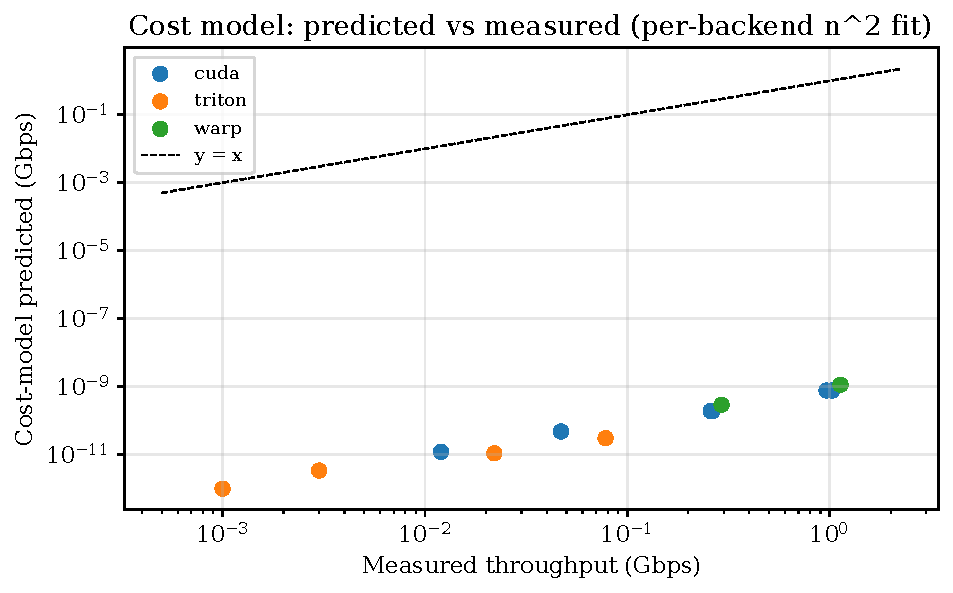
\includegraphics[width=0.86\columnwidth]{fig_costmodel_fit.pdf}
\caption{Cost-model predicted vs measured throughput (per-backend $n^2$ fit); points near
$y{=}x$ indicate the two-parameter model captures the regime.}\label{fig:cm}\end{figure}

\section{Implementation}\label{sec:impl}
A single registry maps a backend/technique to an executor. The NFA is stored once in CSR
and consumed identically by every backend, so comparisons are apples-to-apples.
Correctness is gated against a CPU reference oracle (latch-first-match) and its bit-packed
executable spec.
\textbf{CUDA}: \texttt{dense} (int8/state), \texttt{bitpacked} (register-resident 64-bit
words), \texttt{multistream} (one thread/string), \texttt{multistream\_shared} (CSR staged
in shared memory---a layout Triton cannot express), \texttt{multistream\_async} (pinned +
streamed overlap), and \texttt{worklist} (active-bit iteration via \texttt{\_\_ffsll} +
frontier eps-closure; $O(\text{active})$, no $O(n^2)$), and \texttt{worklist\_global}
(global working set, dynamic word count, no 512-state cap --- scales to ANMLZoo-sized
automata; register residency costs $\sim$4--5$\times$ vs the capped kernel).
\textbf{Triton}: \texttt{dense}, \texttt{bitpacked}, \texttt{multistream},
\texttt{worklist} ($\le 64$ states, via \texttt{libdevice.ffs} + a data-dependent
\texttt{while} loop). \textbf{Warp}: \texttt{multistream} (thread-SIMT Python).
\textbf{Gluon} (Triton's experimental low-level frontend): \texttt{gl.load} always returns
a layout-typed tensor (no scalar load), so the data-dependent CSR inner loop is
inexpressible.

\section{Methodology}
Throughput is measured on a fixed batch ($2048\times256$~B) as total input bits per batch
kernel time, reported as median + percentile-bootstrap 95\% CI over 9 runs (GPU timings
are non-Gaussian~\cite{hoefler}), kernel and transfer time separated. Every configuration
is verified bit-identical to the oracle on examples and randomized fuzz/stress NFAs (up to
500 states). Data and library versions are captured per CSV row. Hardware: NVIDIA RTX 4070
(sm\_89, 46 SMs, 12\,GB); software: CUDA toolkit 13.x, Triton 3.5.1, Warp 1.14, PyTorch
2.9 (cu128). Each datum is the median of 9 batch-kernel times; CSR transitions are read-only
and shared across the batch. We additionally validate on \emph{real} ANMLZoo automata
(Levenshtein 2787 states; Hamming 11349 states, 2.1M transitions; Brill 42661 states, 4.4M
transitions; loaded from pinned public ANML with correct \texttt{all-input}/\texttt{start-of-data}
semantics): \texttt{worklist\_global} matches the reference oracle bit-for-bit on every input,
confirming correctness at production scale (tens of thousands of states).

\section{Results}\label{sec:results}

\begin{table}[t]
\centering
\caption{Throughput (Gbps) by technique and NFA size (batched, RTX 4070). Dashes:
$>64$ states unsupported by the single-word Triton/Warp kernels.}
\label{tab:throughput}
\small
\begin{tabular}{rrrrr}
\toprule
states & CUDA worklist & CUDA full-scan & Triton full-scan & Triton worklist \\
\midrule
32  & 170.2 & 0.513 & 0.071 & 24.4 \\
64  & 163.8 & 0.131 & 0.021 & 25.2 \\
128 & 47.6  & 0.023 & 0.003 & --   \\
256 & 31.7  & 0.006 & 0.001 & --   \\
500 & 15.5  & 0.0015& 0.0002& --   \\
\bottomrule
\end{tabular}
\end{table}

\begin{table}[t]
\centering
\caption{Nsight Compute counters (single launch). Full-scan: SM throughput $\gg$ DRAM
$\Rightarrow$ compute-bound; shared-CSR is identical but for L2 hit rate.}
\label{tab:nsight}
\small
\begin{tabular}{lrrrr}
\toprule
kernel & SM\% & DRAM\% & L2 hit\% & occ\% \\
\midrule
\texttt{multistream} (full-scan) & 19.44 & 0.01 & 79.2 & 16.7 \\
\texttt{multistream\_shared}     & 19.60 & 0.01 & 93.0 & 16.7 \\
\texttt{worklist} (16384 str)    & 5.43  & 6.30 & 95.6 & 23.4 \\
\bottomrule
\end{tabular}
\end{table}

Table~\ref{tab:throughput} reports throughput; Table~\ref{tab:nsight} the Nsight counters.

\textbf{The faithful kernel is compute-bound; memory layout is irrelevant there.}
\texttt{multistream}, \texttt{multistream\_shared} (modeled CSR traffic $=0$), and
\texttt{multistream\_async} tie to within the bootstrap CI at every size
(Fig.~\ref{fig:mem}), and throughput scales as $1/n^2$ (Fig.~\ref{fig:thr}). Nsight Compute
counters confirm this at the hardware level: the full-scan kernel sustains $\approx$19\% of
peak SM throughput but only \textbf{0.01\%} of peak DRAM throughput, and
\texttt{multistream\_shared} shows identical SM\%, DRAM\% and occupancy---only the L2 hit
rate rises (79$\rightarrow$93\%), without moving runtime. The memory axes cannot help until
the algorithm is work-efficient.

\textbf{The work-efficient kernel unlocks the regime.} The \texttt{worklist} kernel is
$250\times$--$10^4\times$ faster than full-scan (the speedup grows with $n$;
Fig.~\ref{fig:wl}) and reaches 15--170~Gbps, moving the workload toward memory-bound where
the memory techniques become load-bearing.

\textbf{Abstraction regret is the execution paradigm.} On the same full-scan kernel the
fitted per-DSL compute cost vs CUDA is Triton $15.7\times$, CUDA $1.0\times$, Warp
$0.62\times$ (Fig.~\ref{fig:regret}). Two equally high-level Python DSLs sit at opposite
extremes: Triton's tile/SPMD paradigm strains to express per-state data-dependent control
flow, Gluon cannot express it at all, while Warp's thread-SIMT model expresses it naturally
and its codegen beats hand-written CUDA.

\textbf{Expressibility $\neq$ efficiency.} Triton \emph{can} express the work-efficient
worklist (unlike Gluon), yet still pays $\approx 9\times$ vs CUDA there (CUDA 142~Gbps vs
Triton 25~Gbps at $\le 64$ states), versus $15.7\times$ on the full scan. Even expressing
the right algorithm, the tile/SPMD model imposes a large constant penalty on scalar,
data-dependent automata work.

\begin{figure}[t]\centering
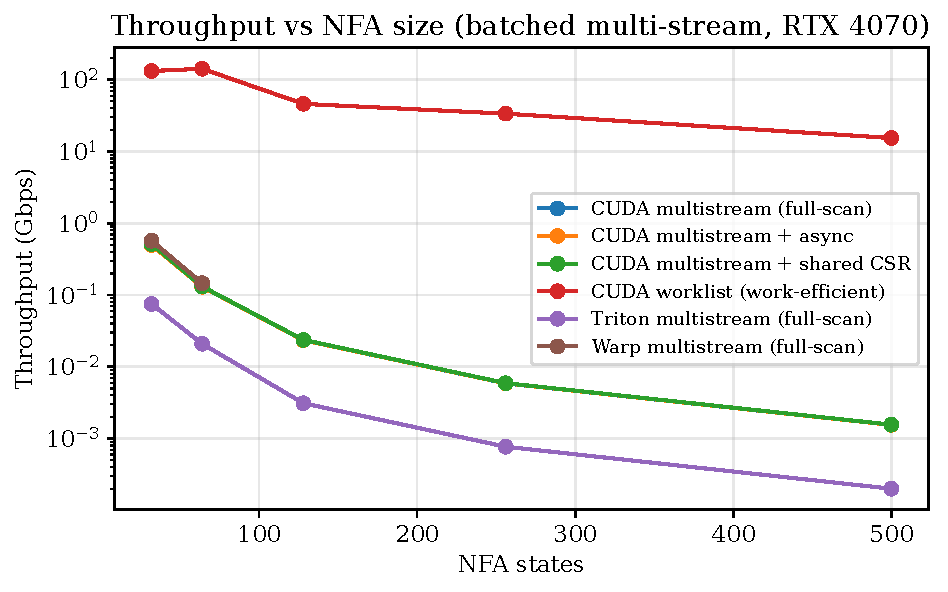
\includegraphics[width=\columnwidth]{fig_throughput_vs_states.pdf}
\caption{Throughput vs NFA size (log scale). Worklist dominates; full-scan techniques
collapse as $1/n^2$.}\label{fig:thr}\end{figure}

\begin{figure}[t]\centering
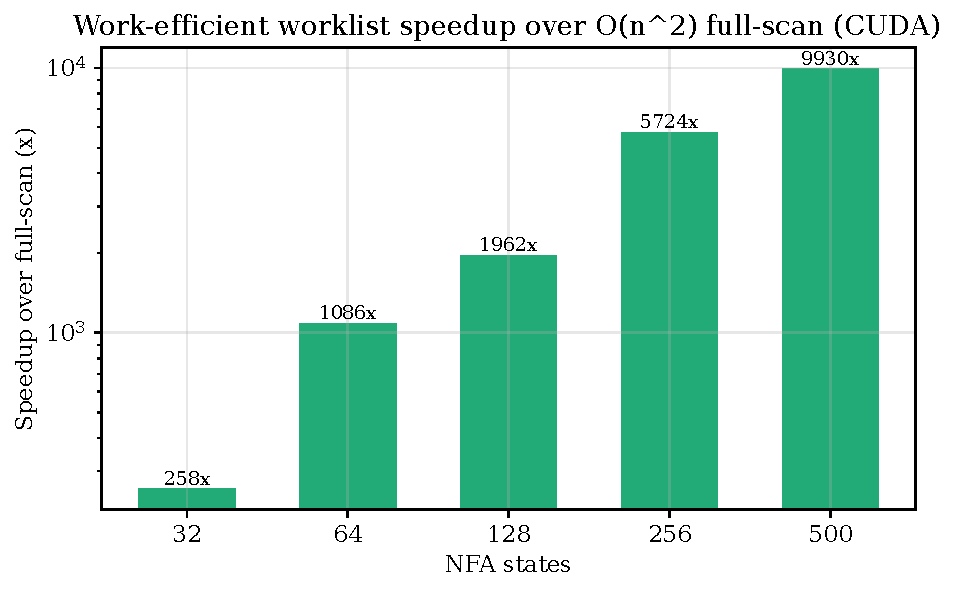
\includegraphics[width=\columnwidth]{fig_worklist_speedup.pdf}
\caption{Work-efficient worklist speedup over $O(n^2)$ full-scan (CUDA), growing with
state count.}\label{fig:wl}\end{figure}

\begin{figure}[t]\centering
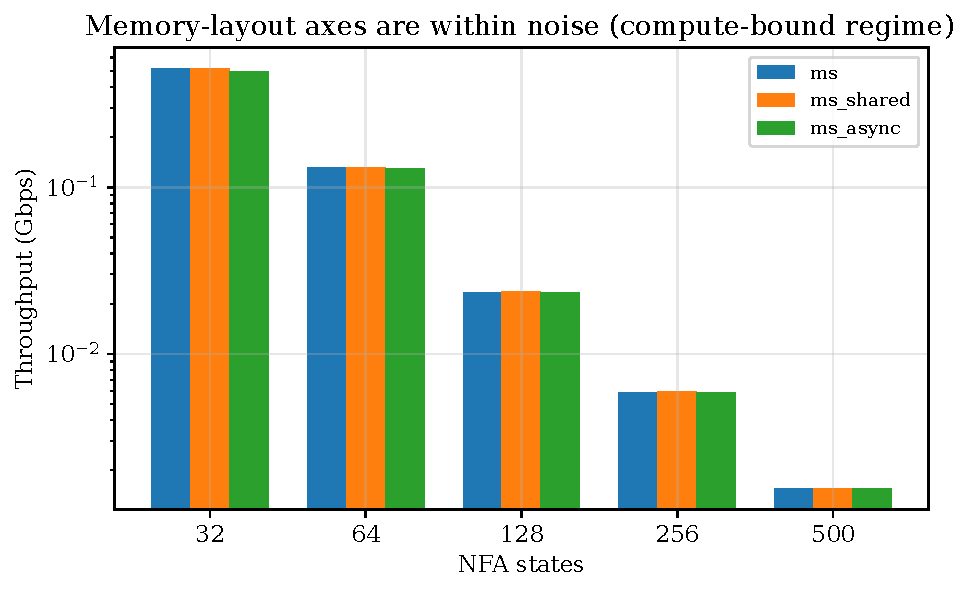
\includegraphics[width=\columnwidth]{fig_memory_ablation.pdf}
\caption{\texttt{multistream} vs \texttt{\_shared} vs \texttt{\_async}: within noise at
every size---compute-bound regime, memory layout irrelevant.}\label{fig:mem}\end{figure}

\begin{figure}[t]\centering
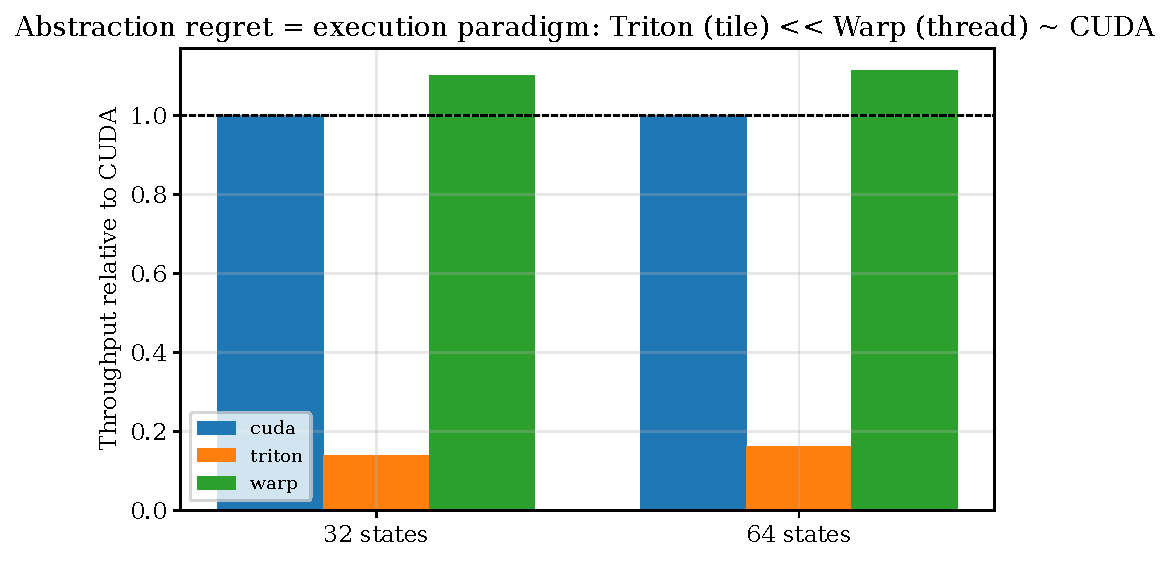
\includegraphics[width=\columnwidth]{fig_abstraction_regret.pdf}
\caption{Throughput relative to CUDA: Triton (tile) $\ll$ Warp (thread) $\approx$ CUDA.
Regret is the execution paradigm, not abstraction height.}\label{fig:regret}\end{figure}

\section{Related work}
Performance portability~\cite{pennycook} measures efficiency across a \emph{hardware set};
abstraction regret measures efficiency across an \emph{abstraction axis at fixed hardware},
attributed to expressibility. The Halide~\cite{halide} lineage established that abstraction
constrains the schedule space; we show the analogous constraint on control flow + memory
layout for irregular automata. SpMV format selection and Gunrock~\cite{gunrock} establish
that layout dominates irregular GPU performance; we add the DSL-expressibility axis. We
rebut the autotuning counter-thesis: our gap is layout/control-flow expressibility, not
tuning---Triton cannot express the shared-CSR layout at any tuning. SOTA automata engines
(ngAP, HybridSA, BitGen) are baselines our worklist engine approaches; our contribution is
the framing + cost model + the multi-DSL expressibility study.

\section{Limitations and future work}
Single GPU architecture so far; a second architecture is needed for generality. The
worklist is one thread/string and, at small batches, under-utilizes the GPU (Nsight: 17\%
occupancy, 2 blocks); a cooperative warp/block-parallel version is the path to SOTA
absolute throughput when streams are few.

\section{Conclusion}
For irregular automata the GPU-DSL promise breaks along a measurable axis we call
abstraction regret, governed by expressibility---of memory layout and, more sharply here,
of data-dependent control flow---not by abstraction height. The memory-organization thesis
holds, but only once the algorithm is work-efficient enough to be memory-bound, which our
worklist engine achieves.

\begin{thebibliography}{1}
\bibitem{infant} N. Cascarano \emph{et al.}, ``iNFAnt: NFA pattern matching on GPGPU
devices,'' \emph{ACM SIGCOMM CCR}, 2010.
\bibitem{asyncap} H. Liu, S. Pai, A. Jog, ``Asynchronous Automata Processing on GPUs,''
\emph{POMACS/SIGMETRICS}, 2023.
\bibitem{ngap} T. Ge, T. Zhang, H. Liu, ``ngAP: Non-blocking Large-scale Automata
Processing on GPUs,'' \emph{ASPLOS}, 2024.
\bibitem{hybridsa} A. Le Glaunec, L. Kong, K. Mamouras, ``HybridSA: GPU Acceleration of
Multi-pattern Regex Matching using Bit Parallelism,'' \emph{OOPSLA}, 2024.
\bibitem{bitgen} T. Ge, X. Chu, H. Liu, ``Interleaved Bitstream Execution for
Multi-Pattern Regex Matching on GPUs,'' \emph{MICRO}, 2025.
\bibitem{hyperscan} X. Wang \emph{et al.}, ``Hyperscan: A Fast Multi-pattern Regex Matcher
for Modern CPUs,'' \emph{USENIX NSDI}, 2019.
\bibitem{anmlzoo} J. Wadden \emph{et al.}, ``ANMLZoo: a benchmark suite for exploring
bottlenecks in automata processing,'' \emph{IISWC}, 2016.
\bibitem{hoefler} T. Hoefler, R. Belli, ``Scientific Benchmarking of Parallel Computing
Systems,'' \emph{SC}, 2015.
\bibitem{pennycook} S. J. Pennycook, J. D. Sewall, V. W. Lee, ``A Metric for Performance
Portability,'' \emph{PMBS@SC / FGCS}, 2016/2019.
\bibitem{halide} J. Ragan-Kelley \emph{et al.}, ``Halide: a language and compiler for
optimizing parallelism, locality, and recomputation,'' \emph{PLDI}, 2013.
\bibitem{gunrock} Y. Wang \emph{et al.}, ``Gunrock: A High-Performance Graph Processing
Library on the GPU,'' \emph{PPoPP}, 2016.
\end{thebibliography}

\end{document}
